\chapter{\mpc, A Language for MPC with Coordination}
\label{ch:mpc}

Busy readers can skip this chapter, returning for details as necessary. The key points from this chapter are
\textbf{(1)} that the informal description of \textbf{Abstractly Sequential} languages in~\Cref{sec:intro-mpc-obliv} is captured
by the~\nameref{thm:mpc-simulation} theorem, and \textbf{(2)} that empirical evidence suggests that
the efficiency of \mpc can be made competitive with traditional MPC languages (e.g. Obliv-C). The implementation
of \system, a Haskell interpreter for \mpc, and \textbf{(2)} is a completed contribution of this proposal.

The purpose of this chapter is to provide a formal description of \mpc and describe our already completed work
on the Haskell implementation, \system.~\Cref{sec:mpc-design} describes \mpc formally, defining the syntax,
sequential semantics, and distributed semantics. These definitions are used to prove~\nameref{thm:mpc-simulation}.
~\Cref{sec:mpc-impl} describes \system, a Haskell interpreter for \mpc. This is a contribution of the proposal.
\system includes both the sequential and distributed semantics, as well as an MPC backend based on EMP~\cite{emp-toolkit}.
It also has additional features not included in the formal model of \mpc. Finally, a set of experiments on a
benchmark suite suggest that performance of \system is similar to Obliv-C. Interested readers can find additional
information on \mpc and \system in~\citet{symphony22}.

\section{Design}
\label{sec:mpc-design}

In addition to the definition of the syntax (\Cref{fig:mpc-syntax}), the formal definition of \mpc
includes two dynamic semantics --- sequential (\Cref{fig:mpc-seq-aux,fig:mpc-seq}) and distributed (\Cref{fig:mpc-dist}).
The sequential semantics represents the local execution of the program, requiring no communication
and no MPC. The distributed semantics represents the distributed execution, requiring communication
between principals performing MPC. The~\nameref{thm:mpc-simulation} theorem ensures that successfully
terminating programs produce the same answer, whether they are executed locally (sequential semantics),
or deployed as a distributed system performing MPC (distributed semantics).

The syntax of \mpc is in \Cref{fig:mpc-syntax}. To simplify the formal semantics,
\mpc is defined using a kind of \emph{administrative normal form} (ANF), meaning
that most expression forms operate directly on variables $x$, rather than subexpressions $e$,
as is the case in the actual implementation.
\footnote{ This restriction does not harm expressiveness. Direct-style syntax like ⸨⦑ref⦒␣(1+⦑read⦒)⸩ can be encoded in \mpc's formal syntax as ⸨⦑let⦒␣x = ⦑read⦒␣⦑in⦒␣⦑let⦒␣y = 1␣⦑in⦒␣⦑let⦒␣z = y+x␣⦑in⦒␣⦑ref⦒␣z⸩. }

\FigureMPCSyntax{fig:mpc-syntax}{\mpc formal syntax.}

\subsection{Standard Expressions}
\label{subsec:mpc-design-standard}

Most of \mpc's expressions are standard. We isolate \emph{atomic expressions} $a$
as a sub-category of full expressions $e$. They include
variables $x$;
integers $i$;
party sets $p$;
binary operations ⸨x ⊙ y⸩ (left abstract, but could be, e.g., addition and multiplication);
multiplexor ⸨x ¿ y ◇ z⸩ (an “if” expression which evaluates both branches and returns one result);
sum injection ⸨ιᵢ␣x⸩ (i.e., tagged union creation);
pair creation ⸨⟨x,y⟩⸩ and projection ⸨πᵢ␣x⸩;
recursive function creation ⸨λ⸤z⸥x⍪ e⸩;
and reference creation ⸨⦑ref⦒␣x⸩ dereference ⸨¡x⸩ and assignment ⸨x ≔ y⸩.
Sum elimination ⸨⦑case⦒␣x␣❴y⍪e⸤1⸥❵␣❴y⍪e⸤2⸥❵⸩ is a full expression ⸨e⸩
because it does not reduce to a value in one step; here, $y$ binds in
the branch bodies $e_i$, only one of which is evaluated.
\footnote{ We can encode ⸨⦑if⦒␣x␣⦑then⦒␣e⸤1⸥␣⦑else⦒␣e⸤2⸥⸩ as
⸨⦑let⦒␣z=0␣⦑in⦒␣⦑let⦒␣y=x ¿ ι₁␣z ◇ ι₂␣z␣⦑in⦒␣⦑case⦒␣y␣❴\_⍪e⸤1⸥❵␣❴\_⍪e⸤2⸥❵⸩. }
Function application ⸨x␣y⸩ and local variable binding ⸨⦑let⦒␣x=e⸤1⸥␣⦑in⦒␣e⸤2⸥⸩
describe full expressions for the same reason. The ⸨⦑par⦒[p]␣e⸩ expression
is specific to the distributed programming setting, which we describe next.

\subsection{Distributed Computing Expressions}
\label{subsec:mpc-design-par}

The \mpc expression ⸨⦑par⦒[x]␣e⸩ says that if $p$ is the
party set contained in variable $x$, then $e$ may be computed at
parties $p$ in parallel (hence the syntax ⸨⦑par⦒⸩). That is, every
party $A \in p$ may evaluate $e$. We say ``may'' here because
nesting such an expression in another ⸨⦑par⦒⸩ could shrink the set of
parties. For example, $e$ in ⸨⦑par⦒[x]␣(⦑par⦒[y]␣e)⸩ will be
evaluated by $p \cap q$ when $y$ is party set $q$; if this
intersection is $\eset$ then $e$ is essentially dead code. The fact that
party sets are \emph{first class} (i.e., can be stored in
variables) and not simply literal annotations allows \mpc
to support rich coordination patterns.

We call the set of parties $m$ computing an expression in parallel
the \emph{mode}. We say the parties $A \in m$ are \emph{present}
for a computation. The semantics of many constructs depends on the
mode. A number $i$ created in mode $m$ is
known only to parties $A \in m$ and notated ⸨i@m⸩. This means that adding two numbers
located at $p$ can only be done in a mode $m$ such that
$m \subseteq p$; if the mode contained additional parties
$A \not\in p$ then they wouldn't know what to do; such states will be
stuck in our semantics. The same goes for functions, sums, and
references. The ⸨⦑read⦒⸩ and ⸨⦑write⦒␣x⸩ expressions perform local
I/O and so can only be run in a mode with a single party.

On the other hand, it is possible that a variable $x$ is in scope for
$A$, but maps to a value only usable by $B$. Party $A$ can
still manipulate a placeholder for $x$ (e.g., to store it in a
data structure or pass it to a function) but may never compute with its
contents (e.g., add to it or branch on it). This approach
simplifies the design of the language at the cost of missing some
(unlikely, but ultimately harmless) logic errors.

\subsection{MPC Expressions}
\label{subsec:mpc-design-mpc}

The \mpc expression ⸨⦑share⦒[x→y]␣z⸩ directs $p$ ($x$'s contents),
required to be a singleton party set, to create secret shares of $z$,
an integer, and distribute the shares to each party in
$q$ ($y$'s contents). All parties $p \cup q$ must be present.
Parties $q$ can all mutually compute on a shared, encrypted value
using ⸨x {⊙} y⸩ and ⸨x {¿} y {◇} z⸩.  Recall from above that the latter is a
multiplexor: we select between ⸨y⸩ and ⸨z⸩ based on whether $x$ is zero or
non-zero. The former models binary operations over numeric types.
An MPC is completed by invoking ⸨⦑reveal⦒[x→y]␣z⸩. This takes $z$, a share
among a set of parties $p$ (the contents of $x$) and converts it to cleartext,
sharing the result among parties $q$ (the contents of $y$). Doing so requires that all of
$p \cup q$ are present so that the shareholders can agree to send the value,
and the result-receivers are ready to receive it.

\subsection{Sequential Semantics}
\label{subsec:mpc-design-seq}

This section defines a small-step, \emph{sequential} (ST)
operational semantics for \mpc. Its execution model treats all
participating parties as if they were executing in lockstep.
We prove that the ST semantics faithfully models the \emph{distributed} (DS)
semantics presented in \Cref{subsec:mpc-design-dist}, according to which parties may act
independently. Thus, the ST semantics can serve as the basis of \mpc formal reasoning,
e.g., about correctness and security.

\FigureMPCSemanticsAux{fig:mpc-seq-aux}{\mpc definitions and metafunctions used in formal semantics.}

\subsubsection{Located Values}
\label{subsubsec:mpc-design-seq-val}

When evaluated, a \mpc expression either loops or returns a \emph{value},
of which their are two kinds. \emph{Located values} ⸨u⸩, defined in
\Cref{fig:mpc-seq-aux}, are only accessible to particular parties. The form
⸨u@m⸩ is a \emph{value}, indicating that the located value ⸨u⸩ is
accessible to each party ⸨A ∈ m⸩, e.g., because it was the result of
evaluating ⸨⦑par⦒[x]␣e⸩ when ⸨x⸩ contained party-set $m$. Values for numbers ⸨i⸢ψ⸣⸩, sets of parties
⸨p⸩, sums ⸨ιᵢ␣v⸩, pairs ⸨⟨v,v⟩⸩, recursive closures ⸨⟨λ⸤z⸥x⍪e,γ⟩⸩ (which include
a closure environment ⸨γ⸩ and “self” binder ⸨z⸩), and memory locations (i.e.,
pointers) ⸨ℓ⸢⋕p⸣⸩ are all located, and otherwise standard except for annotations
⸨ψ⸩ and ⸨⋕p⸩.

For integer values ⸨i⸢ψ⸣⸩, we write just ⸨i⸩ when the annotation ⸨ψ⸩ is~⸨⋅⸩
(i.e., ⸨ψ⸩ is not written at all), and this represents a cleartext value. When
the annotation ⸨ψ⸩ is ⸨⦑enc⦒⋕p⸩ this represents an encrypted value shared among
parties ⸨B ∈ p⸩ (a ``share''). Thus, a value ⸨1⸢⦑enc⦒⋕q⸣@q⸩ can be read as “an
integer 1, encrypted (i.e., secret shared) between parties ⸨q⸩, and accessible to parties
⸨q⸩.” The duplication of ⸨q⸩ may seem redundant, but they may differ
in other contexts. The first ⸨q⸩ represents \emph{among whom is this value shared}
(determined when the share is created), and the second ⸨q⸩ represents
\emph{who has access to this value} (determined by the enclosing ⦑par⦒ blocks).
Location annotations are only used in the sequential semantics in order to
simulate the presence of multiple parties; they are unused in the distributed
semantics and final execution. On the other hand, the ⸨⦑enc⦒⋕q⸩ annotation is
used in distributed execution to detect at runtime buggy programs which fail to
coordinate properly, e.g., if ⸨ A ⸩ attempts to do arithmetic on a secret share
owned by both ⸨ A ⸩ and ⸨ B ⸩, but while ⸨ B ⸩ is not present.

Memory locations ⸨ℓ⸩ are annotated with ⸨⋕p⸩ to indicate the parties
⸨p⸩ that are \emph{co-creators} of the referenced memory. \emph{Values}
are either ⸨u@m⸩ indicating the located value ⸨u⸩ is only accessible to ⸨C ∈ m⸩,
or they are the \emph{opaque value} ⸨★⸩ which indicates the value is both
unknown and inaccessible.

The same figure defines the function ⸨‗↙ₘ⸩, which is used to \emph{(re)locate} a
value to a scope with parties ⸨m⸩ present. For located values ⸨u@p⸩, ⸨‗↙ₘ⸩
relocates them to ⸨p ∩ m⸩, unless the intersection is empty in which case the
value is inaccessible, so it becomes ⸨★⸩. Relocating is a deep operation;
⸨u@p↙ₘ⸩ also relocates the contents ⸨u⸩ to ⸨u↙ₘ⸩, which recurses over
the sub-terms of ⸨u⸩. This step has no effect on closures, though: the closure's
environment's variables get relocated when they are referenced, as we will see.

\FigureMPCSemanticsSequential{fig:mpc-seq}{\mpc sequential semantics.}

\subsubsection{Semantics}
\label{subsubsec:mpc-design-seq-sem}

The small-step, sequential semantics is given in \Cref{fig:mpc-seq}. The
main judgment ⸨ς —→ ς⸩, shown at the bottom, is expressed as rules that step
between \emph{configurations} ⸨ς⸩, which are 5-tuples comprising the current
mode ⸨m⸩, environment ⸨γ⸩, store ⸨δ⸩, stack ⸨κ⸩, and expression ⸨e⸩.
Per~\Cref{fig:mpc-seq-aux}, environments are partial maps from variables to
values, and stores are partial maps from memory locations to values. The main
judgment refers to judgment ⸨γ ⊢ₘ δ,a ↪ δ,v⸩, also shown in the figure, which
defines the evaluation of atomic expressions ⸨a⸩ to values ⸨v⸩.

A stack ⸨κ⸩ is defined by the grammar at the top of
\Cref{fig:mpc-seq}; it is either the empty stack ⸨⊤⸩ or a
list of frames ⸨⟨⦑let⦒␣x=□␣⦑in⦒␣e¦m,γ⟩∷κ⸩. Rule~*⦗ST-LetPush⦘ evaluates
⸨⦑let⦒␣x=e₁␣⦑in⦒␣e₂⸩ by pushing a frame (which includes the skeleton of the
⸨⦑let⦒⸩, the current mode ⸨m⸩, and the environment ⸨γ⸩) and then evaluating
⸨e₁⸩. By rule~*⦗ST-LetPop⦘, when the current expression is atomic, we
evaluate it to a value ⸨v⸩, and then pop the top frame and evaluate its
contents ⸨e₂⸩ in the frame's mode ⸨m⸩ and in its captured environment ⸨γ′⸩
extended with variable ⸨x⸩ mapped to value ⸨v⸩.

The rules satisfy two key invariants. First, if ⸨γ ⊢ₘ δ,a ↪ δ,v⸩ then ⸨v⸩ is «compatible
with» ⸨m⸩. A value ⸨v⸩ is compatible with a set of parties ⸨m⸩ when it is
accessible to some set of parties ⸨p ⊆ m⸩. Formally, the compatibility of ⸨v⸩
with ⸨m⸩ is captured by ⸨v↙ₘ = v⸩; that is, ⸨v⸩ is already located at ⸨m⸩, and
re-locating it there does nothing. (Note that ⸨‗↙ₘ⸩ is idempotent.)
The second invariant is that to \emph{destruct} a value located at ⸨m⸩
requires running in mode ⸨m⸩, i.e., all parties which know the value must be
present. This invariant helps ensure these parties, when running in a
distributed setting with their own store, environment, etc. will agree on the
result.

\paragraph*{Variables, Literals, Binding, and Closures}

Rule~*⦗ST-Var⦘ retrieves a variable's value from the environment and
locates it to the current mode ⸨m⸩ via ⸨γ(x)↙ₘ⸩. Rule~*⦗ST-Lit⦘ evaluates
cleartext constant ⸨i⸩ to the value ⸨i@m⸩, or party set ⸨p⸩ to the value ⸨p@m⸩;
the location is based on the evaluation mode ⸨m⸩.  Rule~*⦗ST-PSetBinop⦘ computes
the union of two party sets in the expected way. Rules~*⦗ST-IntBinop⦘
and~*⦗ST-Mux⦘ capture arithmetic and atomic conditional functions over integers,
but in a way that is parametric in cleartext and encrypted (via multiparty
computation) modalities; we say more, shortly.

Because locations are narrowed when a variable is accessed, we don't need to
explicitly (re)locate a closure's environment ⸨γ⸩ in the relocating
operation in Rule~*⦗ST-Fun⦘. Rule~*⦗ST-App⦘ requires the closure to be available at ⸨m⸩,
the current mode, and sets of evaluation of its body in the standard way.

\paragraph*{Par Mode}

The current mode ⸨m⸩ may change due to ⸨⦑par⦒[x]␣e⸩, which denotes a
sub-computation ⸨e⸩ to be evaluated only by parties in the set stored
in ⸨x⸩; call that set ⸨p⸩. Operationally, ⸨⦑par⦒[x]␣e⸩ evaluates ⸨e⸩ in mode
⸨m ∩ p⸩; i.e., only those parties in ⸨p⸩ which are «also» present in ⸨m⸩ will run ⸨e⸩.
When ⸨m ∩ p⸩ is non-empty, rule~*⦗ST-Par⦘ directs ⸨e⸩ to evaluate in the refined mode.
If ⸨m ∩ p⸩ is empty, then per rule~*⦗ST-ParEmpty⦘, ⸨e⸩ is skipped and ⸨★⸩ is returned.
(Since ⸨★⸩ is a value, not an expression, we return a fresh variable and the
environment with that variable mapped to ⸨★⸩.) Note that because the stack
tracks each frame's mode, when the current expression completes the old
mode will be restored when a stack frame is popped.

\paragraph*{Sums, Pairs, and Party Sets}

Sums and pairs are essentially standard, modulo the consideration of their values' locations.
%
Rule~*⦗ST-Inj⦘ introduces a sum, and rule~*⦗ST-Case⦘ eliminates it, binding the
contents to ⸨x⸩ in the appropriate branch ⸨i ∈ ❴1,2❵⸩, in the usual way.
%
Rule~*⦗ST-Pair⦘ introduces a pair, and rule~*⦗ST-Proj⦘ eliminates it.
%
Party sets can be constructed by set-union in rule~*⦗ST-PSetBinop⦘,
and eliminated in the style of sums using rules~*⦗ST-Case-PSet-Emp⦘
and~*⦗ST-Case-PSet-Cons⦘. The former rule eliminates an empty set,
evaluating to first-branch expression ⸨e₁⸩; the latter rule binds an
arbitrarily chosen singleton principal ⸨❴A❵⸩ from ⸨x₁⸩ to ⸨x₂⸩ and the
remainder ⸨p⸩ to ⸨x₃⸩ when evaluating second-branch ⸨e₂⸩.

\paragraph*{References}

Rule~*⦗ST-Ref⦘ creates a fresh reference in the usual way, returning a located
pointer, but annotated with the parties that created it.
Rule~*⦗ST-Deref⦘ takes a reference located in the current mode ⸨m⸩ and
returns the pointed-to contents made compatible with ⸨m⸩. Rule
*⦗ST-Assign⦘ updates the
store with the new value and returns it, as usual, but only works for
⸨ℓ⸢⋕p⸣⸩ references where ⸨p = m⸩, the current mode. Why? Consider the
following example.

M⁅ Aːl@{␣}l
   A⁅ ⦑par⦒[A,B] & ⦑let⦒␣x=⦑ref⦒␣0␣⦑in⦒
   A⁃            & ⦑let⦒␣‗= (⦑par⦒[A]␣x ≔ 1)␣⦑in⦒
   A⁃            & ⦑let⦒␣y = ¡x␣⦑in⦒␣…
   A⁆
M⁆

The variable ⸨x⸩ initially contains a reference ⸨ℓ⸢⋕❴A,B❵⸣⸩ because it was
created in a context with mode ⸨m=❴A,B❵⸩. Then ⸨x⸩ is assigned to by
⸨ A ⸩ in the ⸨⦑par⦒⸩ expression on the subsequent line. By
rule~*⦗ST-Assign⦘, the creators of the reference ⸨⋕❴A,B❵⸩
must match mode $m$ to proceed, but since $m$ is ⸨❴A❵⸩ the program is stuck.
This is desirable because to proceed would cause the ⸨ A ⸩'s and ⸨ B ⸩'s views
of the computation to get out of sync. When we run this program at each of ⸨ A ⸩ and
⸨ B ⸩ separately, as part of the distributed semantics, on ⸨ A ⸩ we would do the assignment but on
⸨ B ⸩ it would be skipped. As such, on ⸨ A ⸩ the value of ⸨y⸩ would be ⸨1⸩ but on
⸨ B ⸩ it would be ⸨0⸩. If the ⸨…⸩ part of the program were to branch on ⸨y⸩ and
then in one branch do some MPC constructs but not in the other, then the two
parties would fall out of sync.

\paragraph*{I/O}

Rules~*⦗ST-Read⦘ and~*⦗ST-Write⦘ handle I/O. They require that the mode is a
singleton party, and locate the resulting value at the singleton set for that party.
In the semantics, ⦑read⦒ nondeterministically returns any integer,
which over-approximates the behavior of reading a particular integer as input
from the host environment.

\paragraph*{MPC}

The remaining rules cover constructs for MPC, as well as local,
integer-based computations.
%
Rule~*⦗ST-Binop⦘ handles arithmetic integer operations which are supported in
both plaintext and encrypted modes, such as ⸨+⸩ and ⸨×⸩. The protocol
⸨ψ⸩ must be the same for both integer arguments, and it must be compatible with the
current mode ⸨m⸩, per the judgment ⸨⊢ₘ ψ⸩. This judgment (not shown) holds when ⸨ψ⸩ is
either~⸨⋅⸩ or ⸨⦑enc⦒⋕m⸩, that is, both integers are either cleartext or
encrypted values shared among those present in ⸨m⸩. The result depends on the
particular operation ⸨⊙⸩, as determined by the semantic function ⸨⟦‗⟧ ∈ ‹binop›
→ ℤ × ℤ → ℤ ⸩ which we leave opaque.
%\footnote{We assume that other operations can be added,
%  depending on the underlying cryptographic scheme. In GMW,
%  comparisons such as $<$ can be encoded using arithmetic operations.}
Rule~*⦗ST-Mux⦘ is similar to *⦗ST-Binop⦘ and functions as a ternary atomic
conditional; it handles a multiplexor according to the semantic function
⸨‹cond›⸩ where ⸨‹cond›(i₁,i₂,i₃) ≜ i₂⸩ when ⸨i₁ ≠ 0⸩, and ⸨‹cond›(i₁,i₂,i₃) ≜ i₃⸩
when ⸨i₁ = 0⸩.

Party ⸨ A ⸩ can create an encrypted value (i.e., a
secret-share) shared among parties ⸨q⸩ using ⸨⦑share⦒[x₁ → x₂]␣x₃⸩ handled by
rule~*⦗ST-Share⦘. Variable ⸨x₁⸩ must be a singleton set of the input party
⸨p⸩ where ⸨|p|=1⸩; variable ⸨x₂⸩ must be the (nonempty) set of parties
who wild hold shares ⸨q ≠ ∅⸩; and
⸨x₃⸩ must be the input share value known to at least the input party ⸨p′ ⊇ p⸩.
The input party (singleton) set ⸨p⸩ and share parties ⸨q⸩ must all be present in
the mode ⸨m⸩, and no other parties may be present (so ⸨m=p∪q⸩). The input party
must be one of the shareholders (⸨p ⊆ q⸩), so that they are present to provide their secret
input during the reveal if necessary. The resulting value is located at ⸨q⸩, and has protocol
⸨⦑enc⦒⋕q⸩ indicating it is an encrypted value shared among parties ⸨q⸩.

A shared encrypted value is revealed from parties ⸨p⸩ to a nonempty set of
parties ⸨q ≠ ∅⸩ as a cleartext result via the ⸨⦑reveal⦒[x₁→x₂]␣x₃⸩, where ⸨x₁⸩
evaluates to ⸨p⸩ and ⸨x₂⸩ evaluates to ⸨q⸩, and ⸨x₃⸩ evaluates to the encrypted
value, as described by rule~*⦗ST-Reveal⦘. All parties ⸨p⸩ among which ⸨x₃⸩
is shared must be present, as well as the recipients of the value ⸨q⸩, and no
other parties.

\subsection{Distributed Semantics}
\label{subsec:mpc-design-dist}

This section presents \mpc's distributed semantics, modeling the
communication and coordination needed for MPC.

\subsubsection{Configurations}
\label{subsubsec:mpc-design-dist-config}

\FigureMPCSemanticsDistributedSubset{fig:mpc-dist}{\mpc distributed semantics, selected rules.
  Note that judgment ⸨⇡.γ ⊢ₘ ⇡.δ,a ↪ ⇡.δ, ⇡.v⸩ is referred to by the elided rule~*⦗DS-LetPop⦘ of the ⸨⇡.ς
—→⸤A⸥ ⇡.ς⸩ judgment, analogously to the sequential semantics in \Cref{fig:mpc-seq}.}

A \emph{distributed configuration} ⸨ C ⸩ collects the execution states
of the individual parties in an MPC\@. A configuration, defined at the top of
\Cref{fig:mpc-dist}, consists of a finite map from parties to \emph{local configurations} ⸨⇡.ς⸩,
which are 5-tuples consisting of %
\textbf{(1)} a mode ⸨m⸩, %
\textbf{(2)} a local environment ⸨⇡.γ⸩, %
\textbf{(3)} a local store ⸨⇡.δ⸩, %
\textbf{(4)} a local stack ⸨⇡.κ⸩, and %
\textbf{(5)} an expression ⸨e⸩.
Local environments, stores, and stacks are the same as their
single-threaded counterparts except that instead of containing
values ⸨v⸩, they contain «local values» ⸨⇡.v⸩, which lack location
annotations ⸨@m⸩.

For a set of parties ⸨m⸩ wishing to jointly execute program ⸨e⸩, the
initial configuration ⸨C⸤0⸥⸩ will map each party ⸨A ∈ m⸩ to a local
configuration ⸨(m,∅,∅,⊤,e)⸩, where ⸨∅⸩ is the empty function (used for
the empty environment and store), ⸨⊤⸩ is the empty stack, and ⸨e⸩ is
the source program.

\subsubsection{Semantics}
\label{subsubsec:mpc-design-dist-sem}

The distributed semantics ⸨C ↝ C′⸩ uses auxiliary judgments ⸨⇡.γ ⊢ₘ ⇡.δ,a ↪
⇡.δ, ⇡.v⸩ and ⸨⇡.ς —→⸤A⸥ ⇡.ς⸩; these are defined in part in
\Cref{fig:mpc-dist}. The main rule~*⦗DS-Step⦘ is used to execute a single party,
independently of the rest. The rule selects some party $A$'s local
configuration ⸨⇡.ς⸩, steps it to ⸨⇡.ς′⸩, then the incorporates the
latter back into the configuration along with all of the other
configurations $C$ that were not changed. This rule can be used
whenever $A$'s active expression $e$ is anything other than ⸨⦑share⦒⸩ or
⸨⦑reveal⦒⸩, which require synchronizing between multiple parties.
Those two cases use the rules~*⦗DS-Share⦘ and~*⦗DS-Reveal⦘,
respectively, discussed below.

\paragraph*{Non-Synchronizing Expressions} \label{para:mpc-design-dist-sem-nonsync}
%
The rules for ⸨⇡.γ ⊢ₘ ⇡.δ,a ↪ ⇡.δ, ⇡.v⸩ are essentially the same as
those for the single-threaded semantics, except that they operate on
non-located data. The figure shows two examples. Rule~*⦗ST-Var⦘'s
conclusion locates the
result at $m$ via ⸨γ(x)↙ₘ⸩, but rule~*⦗DS-Var⦘'s conclusion simply
returns ⸨⇡.γ(x)⸩. Similarly, rule~*⦗ST-IntBinop⦘'s premise requires
⸨i₁⸢ψ⸣@m = γ(x₁)↙ₘ⸩ while rule~*⦗DS-IntBinop⦘'s premise simply
requires ⸨i₁⸢ψ⸣ = ⇡.γ(x₁)⸩. For elimination forms, a location mismatch
in a single-threaded rule would translate to failed attempt to
eliminate ⸨★⸩ in the distributed rule. For example, if rule~*⦗ST-IntBinop⦘
would have failed because ⸨i₁⸢ψ⸣⸩ was located not at ⸨m⸩ but at ⸨p ⊂
m⸩ instead, then rule~*⦗DS-IntBinop⦘ would fail for parties ⸨A ∈ (m-p)⸩
since for these ⸨⇡.γ(x₁) = ★⸩, which cannot be added to another
share. The check ⸨⊢ₘ ψ⸩ is present in both rules to prevent attempts
to add incompatible shares. Likewise,
rules~*⦗DS-Deref⦘~and~*⦗DS-Assign⦘ (not shown) retain the check from the ST
versions that the reference owners are compatible with $m$.

The rules for ⸨⇡.ς —→⸤A⸥ ⇡.ς⸩ are also essentially the same as their
counterparts for single-threaded ⸨ς —→ ς⸩, with the exception of the rules for
⸨⦑par⦒[x]␣e⸩ expressions. The arrow is annotated with the party ⸨ A ⸩
whose local configuration is executing. This annotation is used by
rules~*⦗DS-Par⦘~and~*⦗DS-ParEmpty⦘, shown in the figure. The first rule evaluates to the
expression $e$ so long as ⸨A ∈ p⸩, where ⸨p = ⇡.γ(x)⸩, updating the
global mode to ⸨m∩p⸩, just as the ST semantics does. The second rule
handles the case when ⸨A ∉ p⸩, thus skipping $e$ and leaving global
mode $m$ as it is, evaluating to result ⸨x′⸩, which is a fresh
variable bound to ⸨★⸩ in ⸨⇡.γ′⸩.

\paragraph*{Synchronizing Expressions}
%
Rules~*⦗DS-Share⦘ and~*⦗DS-Reveal⦘ are used to evaluate expressions
⸨⦑share⦒⸩ and ⸨⦑reveal⦒⸩, respectively. These expressions require
synchronizing between multiple parties, transferring data from one
party to the other(s), and so the rules manipulate multiple local
configurations at once. But they are quite similar to their
single-threaded counterparts.

In the rules we write $C(m)$ to refer to the set of configurations
mapped to by principals ⸨A ∈ m⸩. When we write $C(m).e = e'$, we are
saying that the expression component ($e$) of each configuration in
the set $C(m)$ is equal to expression $e'$. For~*⦗DS-Share⦘, $e'$ is
⸨⦑share⦒[x₁ → x₂]␣x₃⸩ and for~*⦗DS-Reveal⦘ it is ⸨⦑reveal⦒[x₁ →
x₂]␣x₃⸩. We similarly insist that each party's configuration agrees on
the valuation of ⸨x₁⸩ to ⸨p⸩ and ⸨x₂⸩ to ⸨q⸩, which together comprise
the agreed-upon mode $m$. For~*⦗DS-Share⦘, the sharing party $p$ must
be a singleton, and its valuation of ⸨x₃⸩ is a cleartext integer;
for~*⦗DS-Reveal⦘, the valuation of ⸨x₃⸩ for all sharing parties ⸨p⸩
must be an encrypted integer shared amongst those parties. All of
these conditions are sufficient that the actual MPC backend used at
each party is able to sync up properly and begin the encrypted
computation.\footnote{Note that in the actual implementation, each
  party ⸨A ∈ m⸩ merely needs to check that its own view of $m$, $p$,
  and $q$ is consistent per ⸨m=p∪q⸩---if not, as shown in the next
  section, it has landed in a \emph{stuck configuration} and can
  signal that MPC has failed with a type error.} The updated
configuration $C'$ matches the original
configuration $C$ but updates the local configuration for each party
⸨A ∈ m⸩ to have expression component $x$, where $x$ is a fresh
variable added to the store ⸨⇡.γ⸩ to map to the communicated
(cleartext or encrypted) integer; those sharing parties ⸨A ∈ p⸩ such
that ⸨A ∉ q⸩ evaluate to ⸨★⸩ instead.

\subsection{Simulation}
\label{subsec:mpc-design-sim}

This section sketches a proof of~\nameref{thm:mpc-simulation} which states
the sense in which we can interpret a \mpc program in terms of its
sequential semantics, even though in reality it will execute in a
distributed fashion.

\FigureMPCSemanticsDistributedAux{fig:mpc-dist-aux}{
  Slicing metafunction used to relate sequential and distributed semantics.}

We can relate a sequential configuration ⸨ς⸩ to a distributed one by
«slicing» it, written ⸨ς↯⸩, which is defined in \Cref{fig:mpc-dist-aux}. Each
party ⸨ A ⸩ in the mode ⸨m⸩ of ⸨ς⸩ is mapped to a 5-tuple that represents its
local state; this local state consists of $m$, $e$, and the sliced
versions of the environment
⸨γ⸩, store ⸨δ⸩, and stack ⸨κ⸩ of ⸨ς⸩ that are specific to ⸨ A ⸩. Slicing is an
otherwise structure preserving operation, but where located values ⸨u@p⸩ are
sliced either to the sliced version of ⸨u⸩ if ⸨A ∈ p⸩ or ⸨★⸩ otherwise. Slicing
captures the simple idea that for a value ⸨u@p⸩, if ⸨A ∈ p⸩ then ⸨ A ⸩ can
access ⸨u⸩, but if ⸨A ∉ p⸩ then it cannot. Note that
shares ⸨i⸢ψ⸣⸩ and locations ⸨ℓ⸢⋕m⸣⸩ are left alone, since they are
needed by the distributed semantics---only the
location annotation is affected.

To capture the relationship between sequential and distributed execution
models we prove a semantic correspondence theorem between them, which is
slightly weaker than full bisimulation. The proof of the theorems follow
from two key lemmas: «forward simulation» and «confluence». Forward simulation
establishes that for every sequential execution, there exists a compatible distributed
one. Confluence establishes taht even though the distributed semantics is nondeterministic,
its final states are uniquely determined.

A «successful termination» is an execution trace that
concludes in a «terminal state», defined as:

M⁅ Aːrcl
   A⁅ ⟪⸨ς⸩ is a terminal state⟫   ⧼⇡△⟺⧽ ς = m,γ,δ,⊤,a ∧ γ ⊢ₘ δ,a ↪ δ′,v
   A⁃ ⟪⸨⇡.ς⸩ is a terminal state⟫ ⧼⇡△⟺⧽ ⇡.ς = m,⇡.γ,⇡.δ,⊤,a ∧ ⇡.γ ⊢ₘ ⇡.δ,a ↪ ⇡.δ′,⇡.v
   A⁃ ⟪⸨ C ⸩ is a terminal state⟫   ⧼⇡△⟺⧽ ∀ A ∈ ‹dom›(C)⍪ ⟪⸨C(A)⸩ is a terminal state⟫
   A⁆
   M⁆

This definition captures the idea that a state is terminal if the execution
stack is empty (⸨⊤⸩), the next term to execute is atomic (⸨a⸩), and the
atomic expression is able to step (via ⸨↪⸩) to a value ⸨v⸩.
There are no successor configurations which can be reached from a terminal state. Any
state which is both non-terminal and also has no successor configurations we
call «stuck». Given this definition of terminal states, we are ready to
state~\nameref{thm:mpc-simulation}:

\begin{theorem}[Simulation (\mpc)]\label{thm:mpc-simulation}
  If ⸨ς —→⋆ ς'⸩ then ⸨ς′⸩ is a terminal state and ⸨C = ς'↯⸩ ⸨⟺⸩ ⸨ς↯ ↝⋆ C ⸩ and ⸨ C ⸩ is a terminal state.
\end{theorem}

A crucial aspect of the correspondence is that it only
holds for «successfully terminating» executions. This means the correspondence
 does not capture executions which diverge or get stuck due to runtime failure,
 e.g., a configuration will get stuck if ⸨ A ⸩ attempts to create a secret share
 with ⸨ B ⸩ when ⸨ B ⸩ is not present in the computation.

\section{Implementation}
\label{sec:mpc-impl}

The interpreter for \mpc, \system, was implemented in 4K lines of Haskell. The
interpreter can run programs in sequential mode for prototyping and debugging,
and distributed mode for actual MPC\@.
%
Full \system adds a number of features beyond \mpc, including booleans and a conditional
expression; nested pattern-matching on pairs, sums, lists, principal
sets and bundles;
arrays (immutable vectors with O(1) lookup); and
non-local control flow (e.g., early return).

The \system interpreter provides a general interface for MPC
protocols. The ⸨⦑share⦒⸩ primitive is extended thus:
⸨⦑share⦒[φ,τ:P→Q]␣v⸩. Here, the metavariable ⸨φ⸩ denotes protocols
(e.g., ⸨⦑yao⦒⸩) and the metavariable ⸨τ⸩ denotes types. A
particular protocol implementation must provide operations for creating, combining,
and revealing shares. Shares are an abstract data type, so each protocol is free to
choose their own representation. So far we have only implemented
two-party Yao's garbled circuits, linking to the EMP toolkit~\cite{emp-toolkit}.
The share ADT for Yao the protocol is a foreign pointer to
an EMP C++ object. All MPC operations on primitive types (i.e. booleans,
naturals, integers, and floats) are implemented via FFI to their
corresponding operations in C++. We are currently working on adding
support for an N-party GMW backend.

The interpreter also generalizes \mpc
by allowing ⸨⦑mux⦒⸩, ⸨⦑case⦒⸩, ⸨⦑share⦒⸩ and ⸨⦑reveal⦒⸩ to operate
recursively over on pairs, sums, and lists. It adds another expression,
⸨⦑mux-case⦒⸩, for case analysis on encrypted sums, which are
represented with pairs: \mpc value ⸨ι₀␣v⸩ is represented
⸨⟨⦑true⦒,⟨v,⦑default⦒⟩⟩⸩ and value ⸨ι₁␣v⸩ is represented
⸨⟨⦑false⦒,⟨⦑default⦒,v⟩⟩⸩, with each of the components encrypted. The value
⸨⦑default⦒⸩ is to allow case analysis to proceed on \emph{both} branches of
⸨⦑mux-case⦒⸩, as a kind of multiplexor. The precise value of ⸨⦑default⦒⸩ is
determined when sharing, based on the type annotation on
⸨⦑share⦒[φ{,}τ{:}P{→}Q]␣⦑default⦒⸩.

The expressiveness of \system{} enables us to implement many convenient data structures
and coordination patterns as libraries. We provide a standard library (about 800 LOC) for \system{}
including (but not limited to) libraries for coordination (e.g., initializing a bundle from a principal
set) and bounded recursion (for unrolling an MPC function).

\subsection{Experimental Evaluation}
\label{subsec:mpc-impl-eval}

We evaluate \system for two reasons.
The first is to demonstrate \system's expressivity.
We do so by implementing interesting benchmark programs.
The second is to demonstrate that Symphony does not introduce unreasonable performance overhead.
We have argued that Symphony is highly expressive, but it is
important that expressivity not come at significant performance cost.
Our experiments show that Symphony, while slower than one state-of-the-art tool,
is performant.

\paragraph{Experimental Setup}

To evaluate performance we compare \system with
OblivC~\cite{cryptoeprint:2015:1153}.
For fair comparison, both languages were configured to use EMP as their
MPC backend; we extended OblivC to use EMP via its
callback interface.

We used both \system and OblivC to implement a benchmark suite of five
programs:
\begin{itemize}
  \item \texttt{hamming} (from~\cite{10.1007/978-3-642-54807-9_15, CCS:ZhaSteBla13}, 12 LOC app, 0 LOC lib) finds the Hamming distance of two strings.
  \item \texttt{bio-match} (from~\cite{CCS:BDKKS18}, 20
LOC app, 16 LOC lib) finds the minimum Euclidean distance between a set of points
(from ⸨ A ⸩) and a single point (from ⸨ B ⸩) in 2D space.
  \item \texttt{db-analytics} (from~\cite{CCS:BDKKS18}, 35 LOC app, 8 LOC lib) computes the mean
    and variance over the union and join of two databases.
  \item \texttt{gcd-gc} (from~\cite{10.1145/3319535.3339818}, 11 LOC app, 11 LOC lib) determines the GCD of two numbers using Euclid's algorithm.
  \item \texttt{edit-dist} (from~\cite{cryptoeprint:2015:1153}, 26 LOC app, 20 LOC lib) computes the edit distance, by dynamic
    programming, between two strings.
\end{itemize}
We have also implemented trivial ORAM~\cite{10.1145/2810103.2813634}, insertion sort, and k-means~\cite{CCS:BDKKS18} in \system (but did not compare them against OblivC).

Experiments were run on a 2019 MacBook Pro with a 2.8 GHz Quad-Core
Intel Core i7 and 16GB of RAM (OSX 11.3.1).
Experiments were run on two simulated networks:
a LAN (1Gbps bandwidth, ⸨<⸩1ms RTT latency) and a WAN (100Mbps bandwidth, 50ms RTT latency).
All experiments use 32-bit integers, except for \texttt{gcd-gc}
which uses 64-bit integers.
Reported execution times measure the end-to-end execution time of party ⸨ A ⸩ and were averaged over five samples.

\begin{figure*}
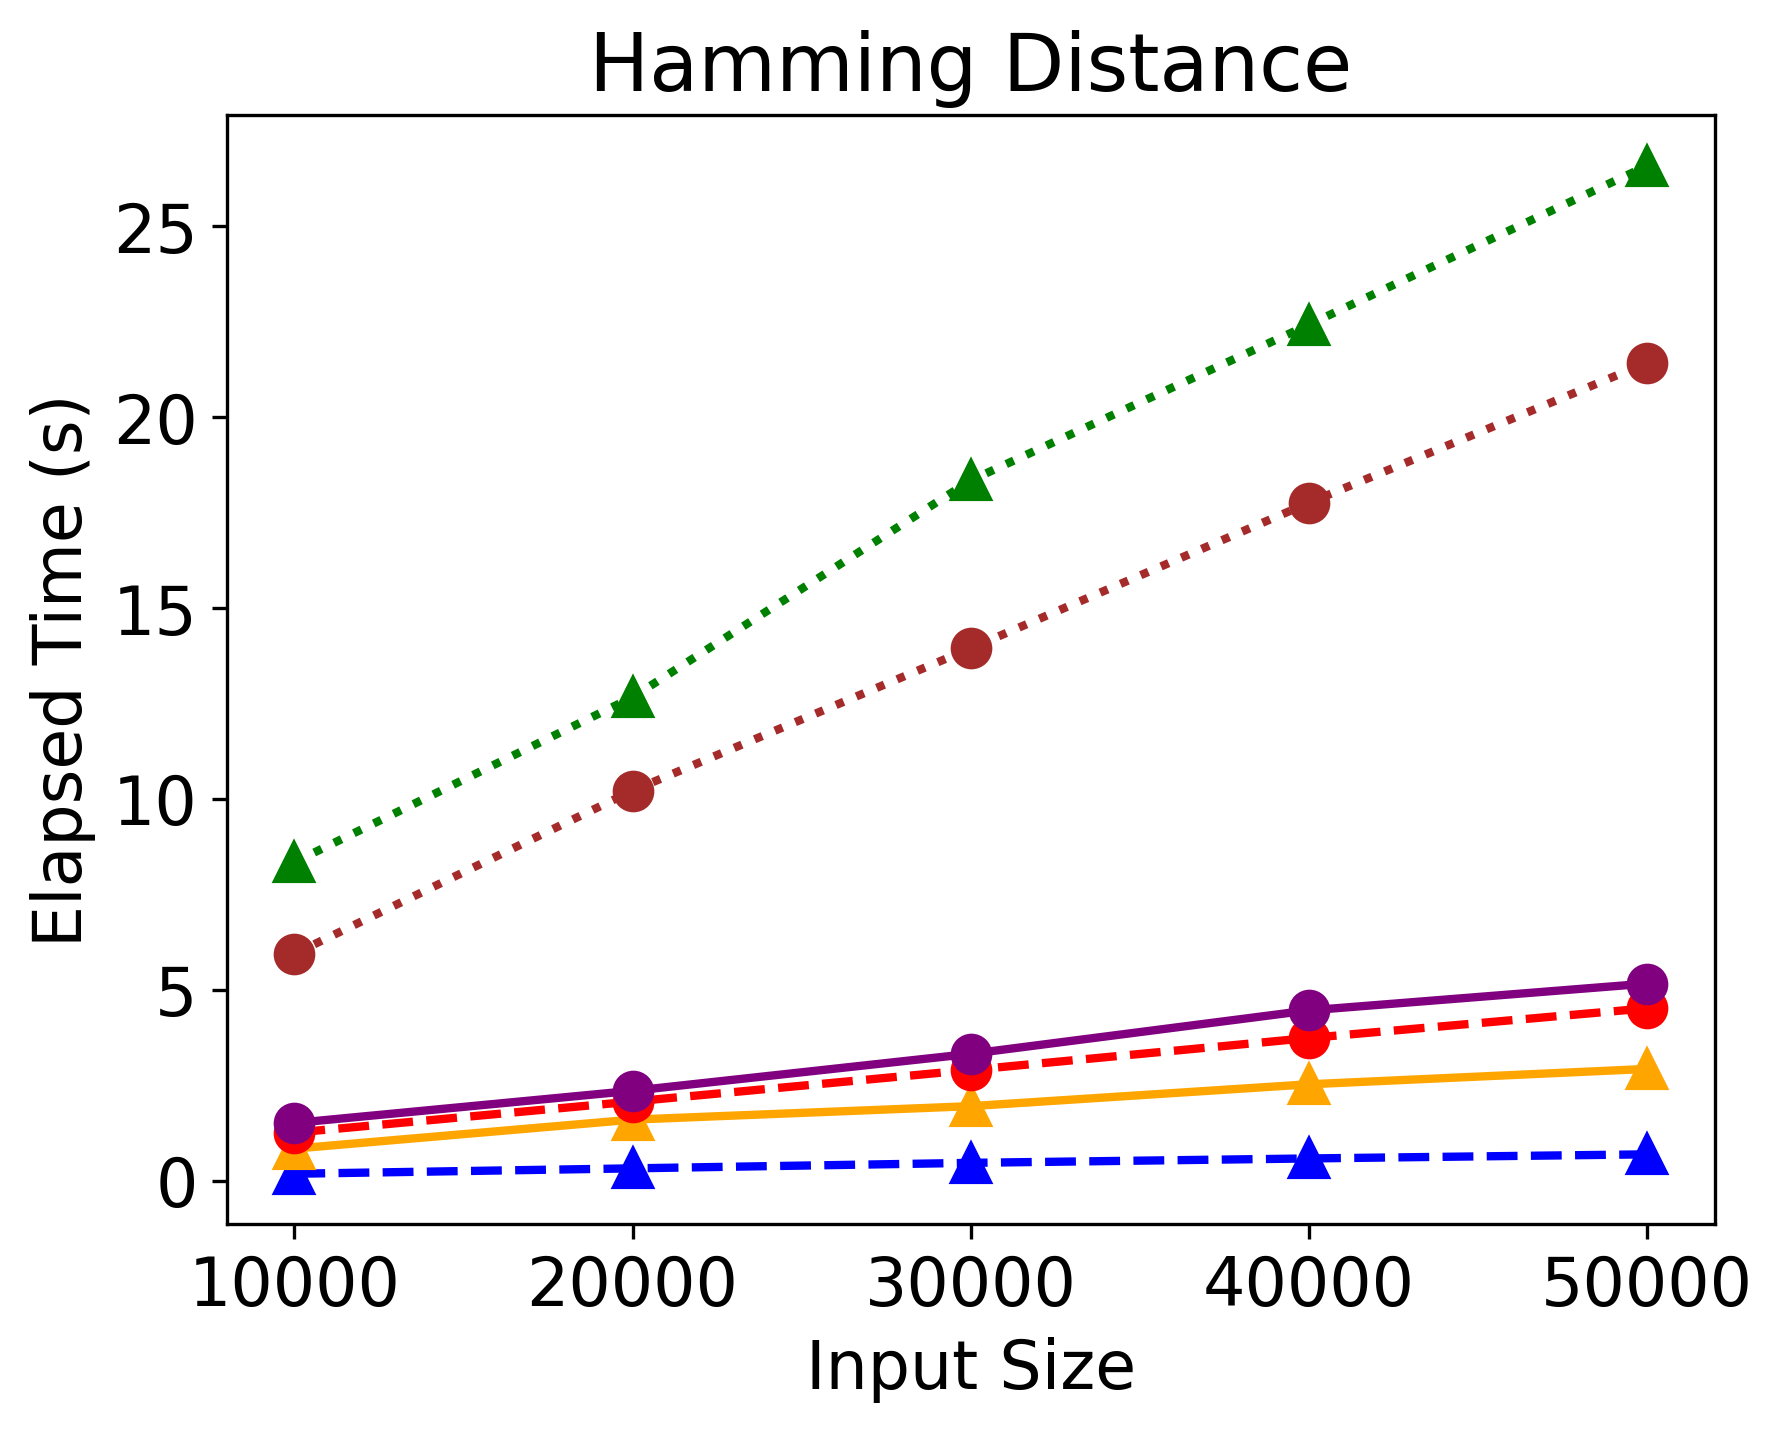
\includegraphics[width=.33\linewidth,align=t]{../figures/hamming.png}
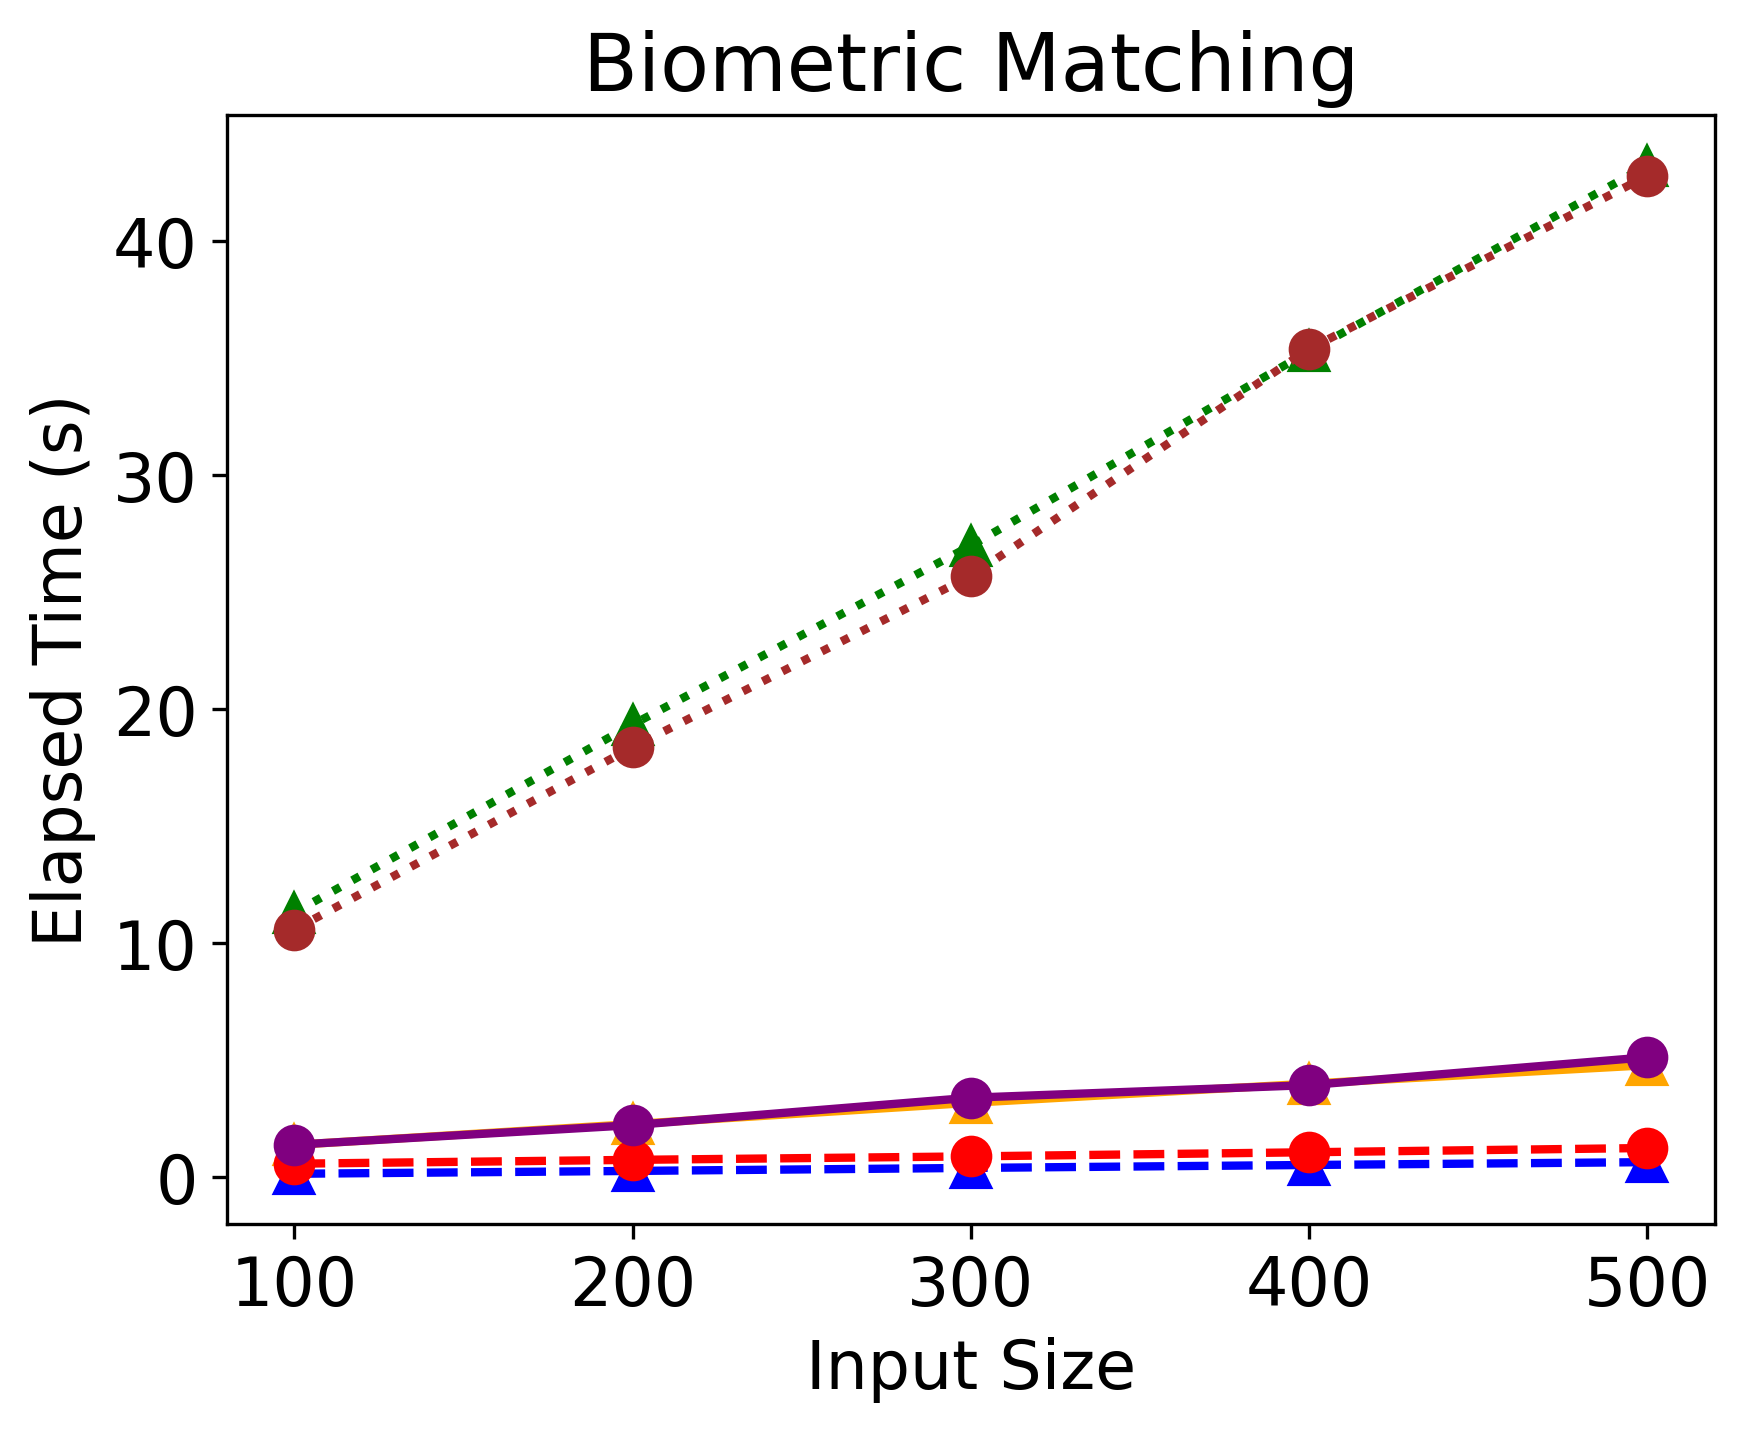
\includegraphics[width=.33\linewidth,align=t]{../figures/bio-matching.png}
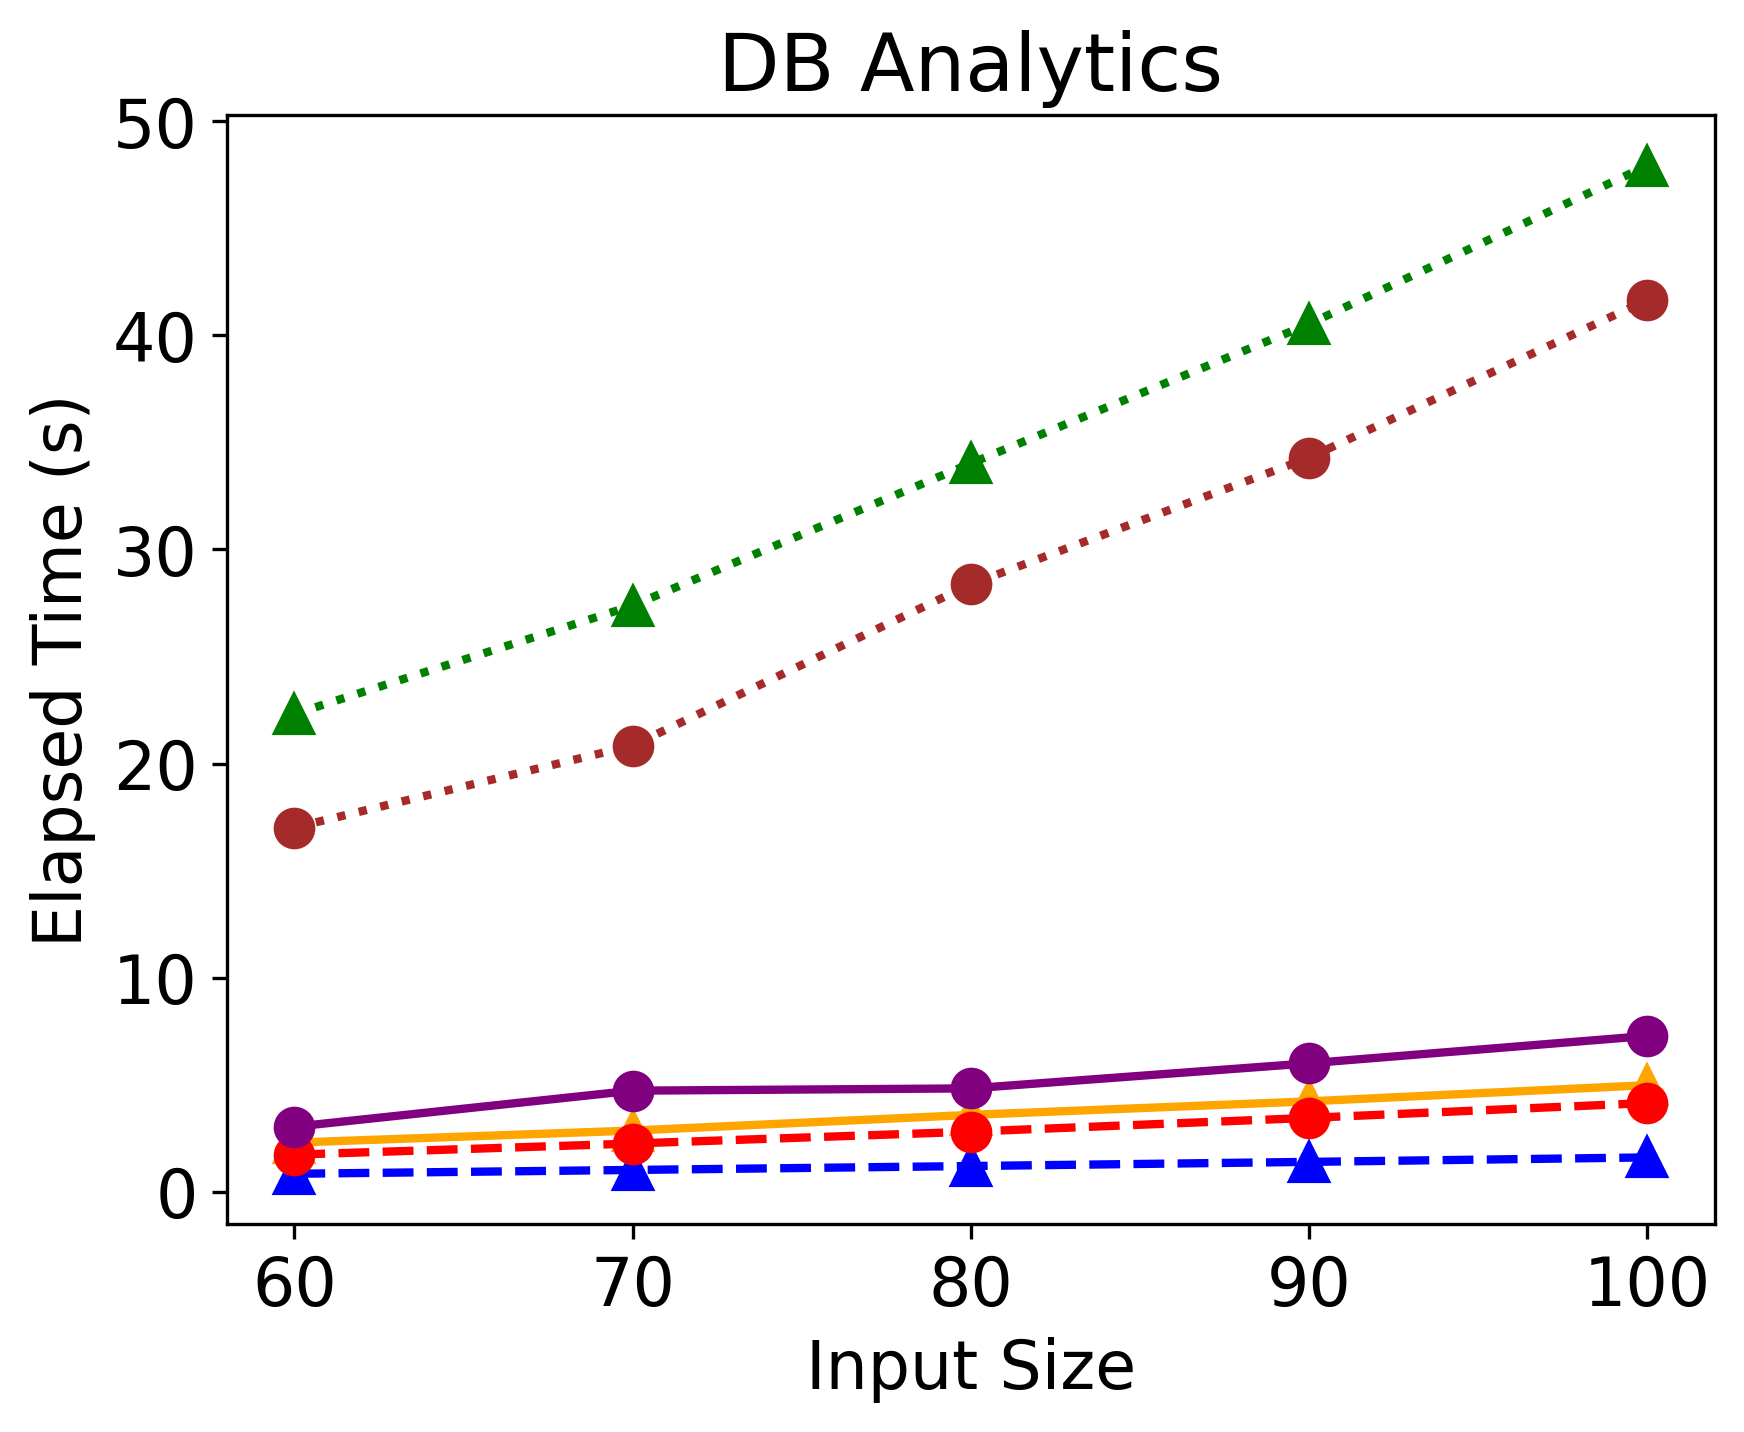
\includegraphics[width=.33\linewidth,align=t]{../figures/db-analytics.png}
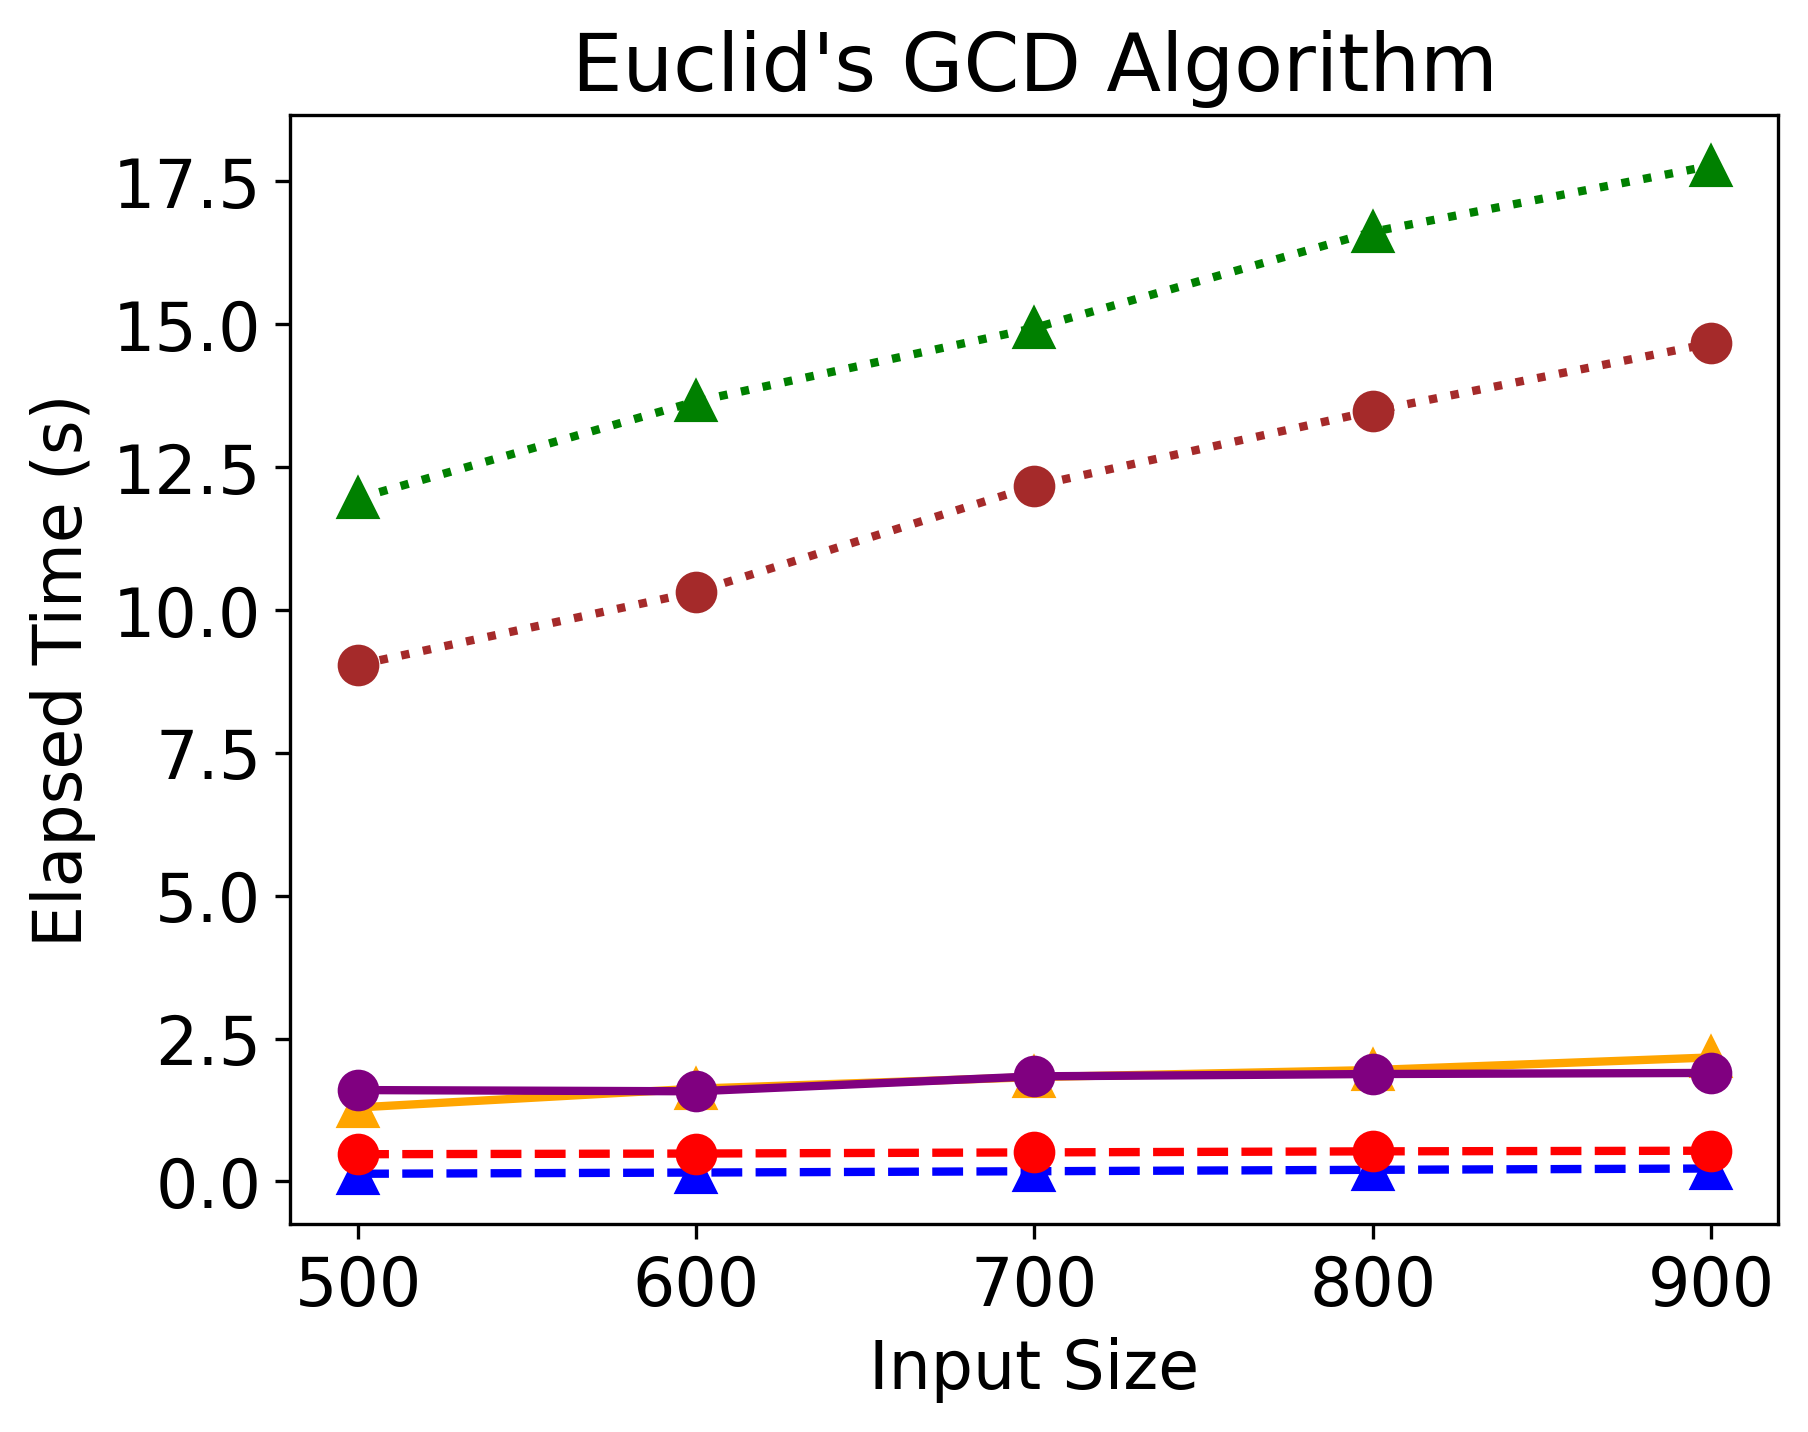
\includegraphics[width=.33\linewidth,align=t]{../figures/gcd-gc.png}
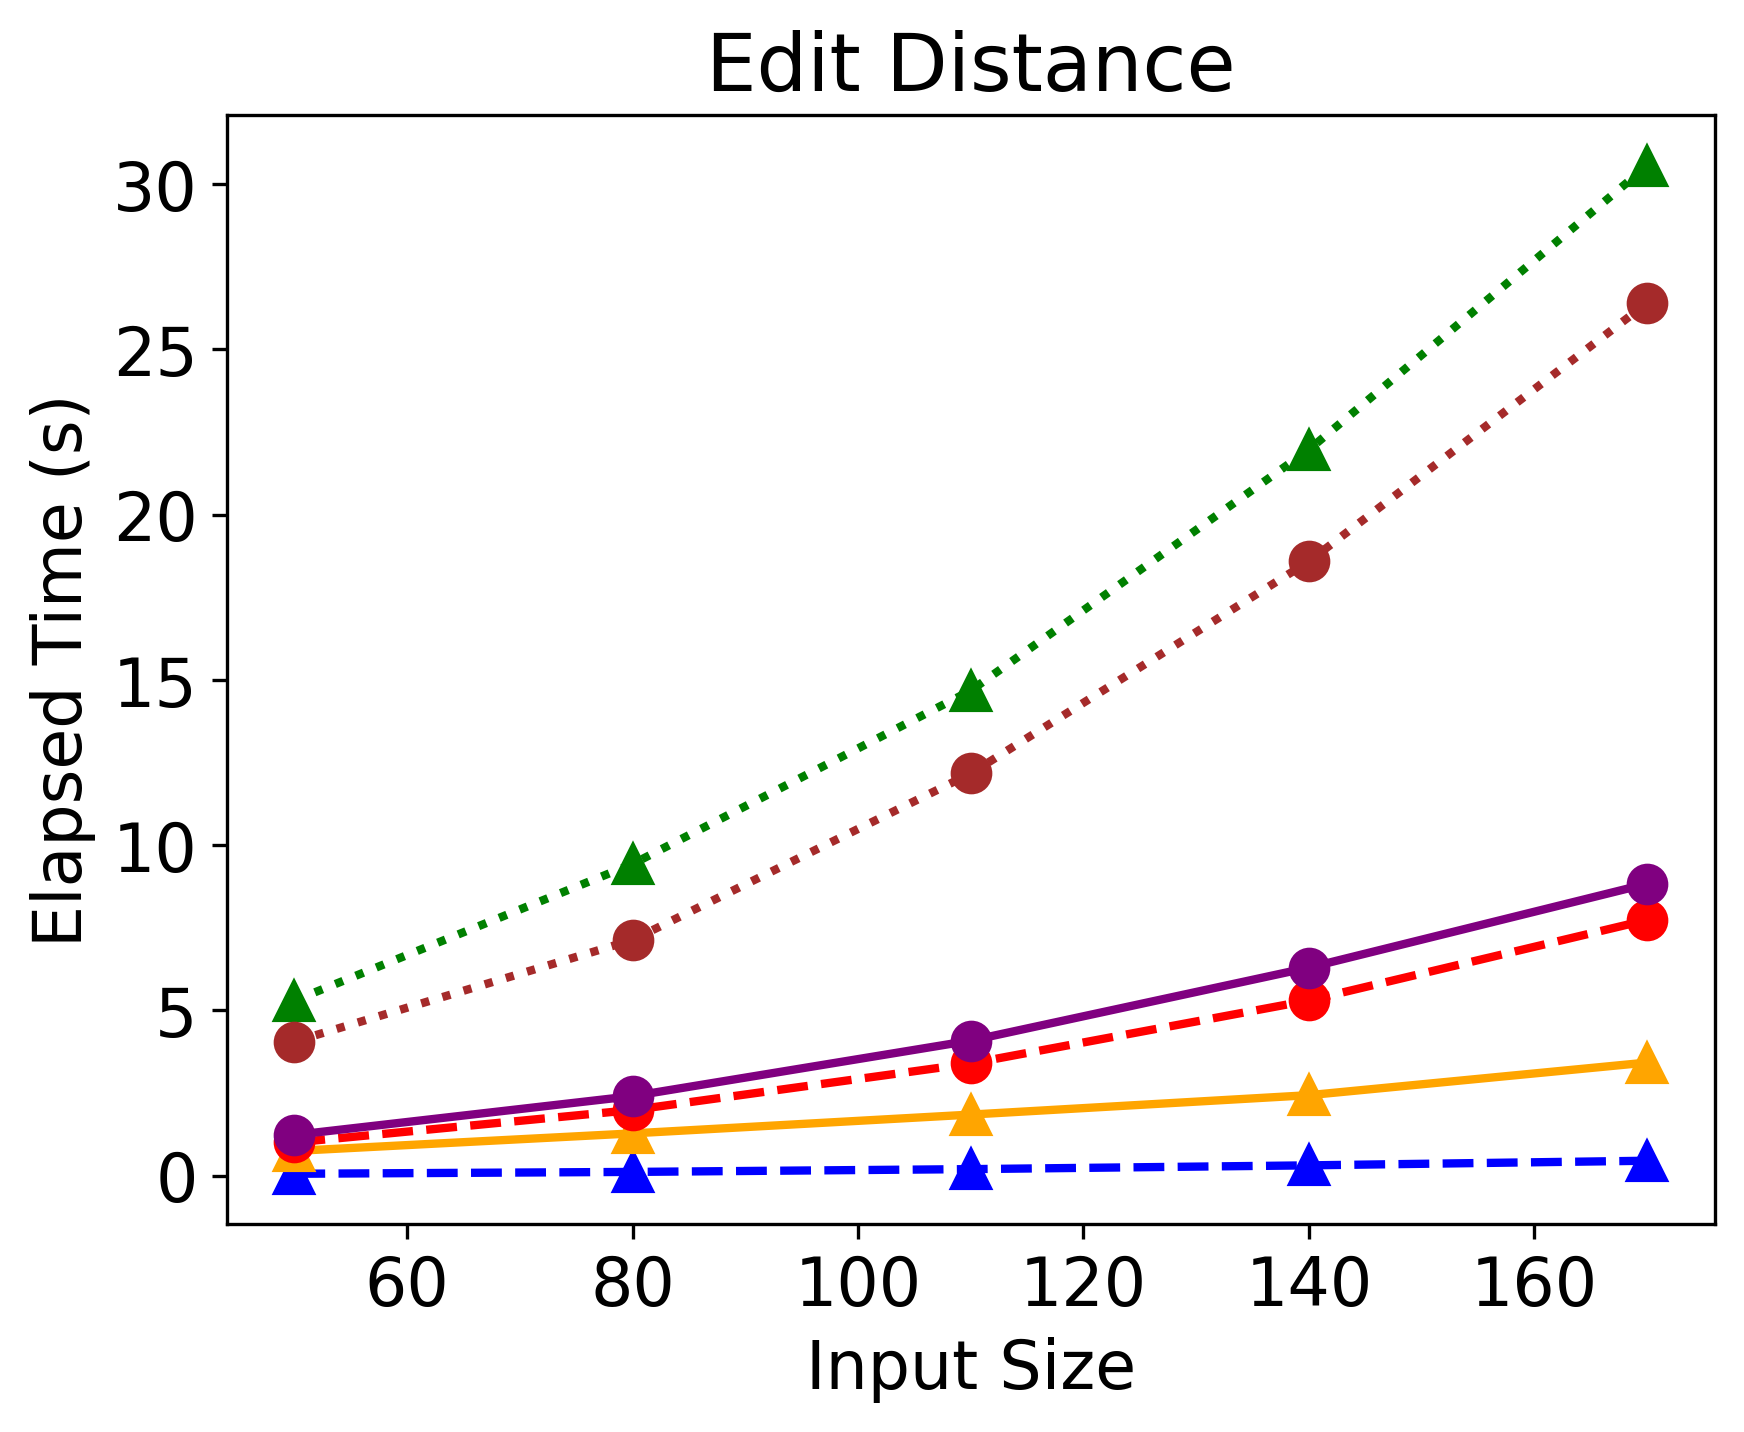
\includegraphics[width=.33\linewidth,align=t]{../figures/edit-distance.png}
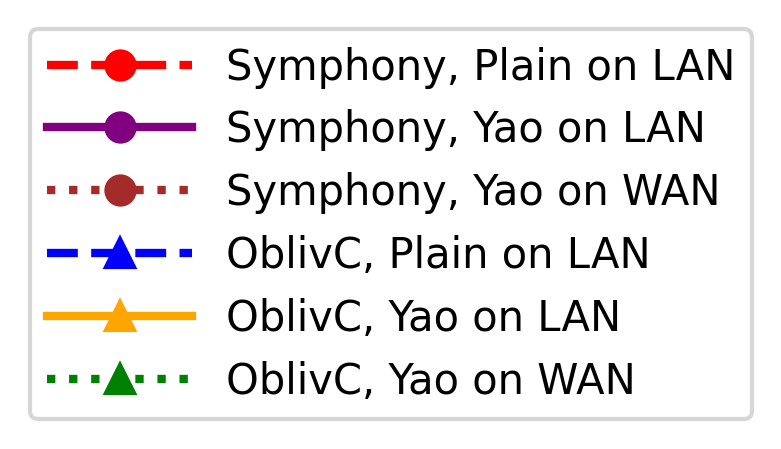
\includegraphics[width=.265\linewidth,align=t]{../figures/legend.png}
\caption{%
  End-to-end execution time (in seconds) of benchmarks, averaged over five samples.
  \textbf{LAN} is a simulated 1gbps connection with no delay. \textbf{WAN} is a simulated 100Mbps
  connection with a 50ms RTT latency. \textbf{Yao} and \textbf{Plain} protocols use EMP's \texttt{sh2pc}
  (semi-honest, two-party) and \texttt{plain} protocols respectively. \system{} uses EMP's Integer
  interface. OblivC uses EMP's Bit interface (compiling integer operations to circuits).
  Input sizes for all the benchmarks indicate the
  length of the list(s) provided as input, except for \texttt{gcd-gc} where the input size indicates
  the number of iterations of the GCD algorithm.
}\label{fig:mpc-impl-eval-etoe}
\end{figure*}

\paragraph{Runtime Performance}

Figure~\ref{fig:mpc-impl-eval-etoe} plots the end-to-end execution time of \system{}
and OblivC on the benchmarks. These results suggest that, as compared to OblivC,
\system imposes acceptable overhead. There are two primary sources for this overhead:

First, \system supports arbitrary numbers of parties while OblivC supports only two.
      This is significant because \system performs frequent runtime checks on the parties in scope.
      Since \system supports an arbitrary number of possible parties, we
      represent the parties in scope as a set (implemented by a balanced tree
      data structure).
      Thus checks on principals are implemented by set operations.
      OblivC also performs certain checks on parties but, since only two
      parties are supported, these are implemented as simple integer equality
      checks.

Second, our \system programs use linked lists and pattern matching while our
OblivC programs use arrays.  We believe that this is the dominant source of
overhead, and can be mitigated by rewriting \system programs to use arrays.

Comparing the LAN and WAN benchmarks confirms that the language overhead imposed by \system{} is dominated by
the time it takes to perform network communication during a WAN deployment of MPC. We believe \system{} is faster than OblivC in the WAN setting
due to its use of the EMP Integer interface, which uses the network
more efficiently than the Bit interface used by OblivC's callback
mechanism, and consequently the EMP backend for OblivC.

\paragraph{Generated Circuit Sizes}

\begin{table*}
  \centering
  \smaller
\begin{tabular}{ l l l l l l l l }
\hline \hline
& & \multicolumn{2}{c}{OblivC} & \multicolumn{2}{c}{\system{}} & \multicolumn{2}{c}{$\Delta$ (OblivC - \system{})} \\
\cmidrule(lr){3-4} \cmidrule(lr){5-6} \cmidrule(l){7-8}
Benchmark & Input Size & AND Gates & XOR Gates & AND Gates & XOR Gates & AND Gates & XOR Gates \\
\hline
Hamming Dist. & 10000 & 1249875  & 3159595  & 950000   & 2550000  & 299875  & 609595   \\
              & 20000 & 2499875  & 6319595  & 1900000  & 5100000  & 599875  & 1219595  \\
              & 30000 & 3749875  & 9479595  & 2850000  & 7650000  & 899875  & 1829595  \\
              & 40000 & 4999875  & 12639595 & 3800000  & 10200000 & 1199875 & 2439595  \\
              & 50000 & 6249875  & 15799595 & 4750000  & 12750000 & 1499875 & 3049595  \\
\hline
Bio. Matching & 100   & 2617868  & 6353496  & 2675500  & 8007000  & -57632  & -1653504 \\
              & 200   & 5235768  & 12706996 & 5351000  & 16014000 & -115232 & -3307004 \\
              & 300   & 7853668  & 19060496 & 8026500  & 24021000 & -172832 & -4960504 \\
              & 400   & 10471568 & 25413996 & 10702000 & 32028000 & -230432 & -6614004 \\
              & 500   & 13089468 & 31767496 & 13377500 & 40035000 & -288032 & -8267504 \\
\hline
DB Analytics  & 60    & 4609304  & 9569553  & 4732457  & 10425422 & -123153 & -855869  \\
              & 70    & 6246968  & 12970159 & 6413597  & 14128242 & -166629 & -1158083 \\
              & 80    & 8133020  & 16886701 & 8349937  & 18393262 & -216917 & -1506561 \\
              & 90    & 10268008 & 21320663 & 10541477 & 23220482 & -273469 & -1899819 \\
              & 100   & 12651370 & 26270229 & 12988217 & 28609902 & -336847 & -2339673 \\
\hline
GCD           & 500   & 2360091  & 6735821  & 2302192  & 6910016  & 57899   & -174195  \\
              & 600   & 2832991  & 8085621  & 2762592  & 8291916  & 70399   & -206295  \\
              & 700   & 3305891  & 9435421  & 3222992  & 9673816  & 82899   & -238395  \\
              & 800   & 3778791  & 10785221 & 3683392  & 11055716 & 95399   & -270495  \\
              & 900   & 4251691  & 12135021 & 4143792  & 12437616 & 107899  & -302595  \\
\hline
Edit Dist.    & 50    & 780882   & 1704539  & 637372   & 1779607  & 143510  & -75068   \\
              & 80    & 2003142  & 4378936  & 1631872  & 4556407  & 371270  & -177471  \\
              & 110   & 3790602  & 8291824  & 3085372  & 8614807  & 705230  & -322983  \\
              & 140   & 6143262  & 13443100 & 4997872  & 13954807 & 1145390 & -511707  \\
              & 170   & 9061122  & 19832759 & 7369372  & 20576407 & 1691750 & -743648  \\
\hline
\end{tabular}
\caption{%
  \textnormal{
  Gate counts (AND and XOR) of select benchmark programs. \textbf{Input Size} for Hamming Dist.,
  Bio. Matching, DB Analytics, and Edit Dist. is the length of the input lists. For GCD, it is
  the maximum number of GCD iterations. Gate counts were collected by modifying EMP to record
  AND or XOR gate execution. \system{} uses EMP's Integer interface where applicable,
  OblivC uses EMP's Bit interface (compiling integer operations to circuits).
  }
}
\label{tab:mpc-impl-eval-gates}
\end{table*}

As a second experiment, we instrumented the EMP backend to count the number of utilized AND and XOR gates.
Counting gates is primarily a sanity check that ensures \system is not
erroneously introducing large numbers of unneeded gates.
~\Cref{tab:mpc-impl-eval-gates} tabulates the number of
AND and XOR gates generated by \system{} and by OblivC.
The gate counts generated by \system{} and
OblivC are very similar, with differences caused by using the EMP
Integer interface vs OblivC compiling to the Bit interface (as
required by its callback mechanism. The optimizations
performed by EMP's circuit compiler and OblivC's circuit compiler are similar,
but not identical.

\paragraph{Experimental Conclusions}
Overall, our experiments indicate that the langauge design itself does not
impose significant overhead on either end-to-end execution time or generated
circuit sizes.
At the same time, \system{} is more expressive than frameworks like
OblivC (e.g., by allowing $N$ parties interleave many secure and cleartext computations)
and safer (e.g., by guaranteeing that the distributed deployment matches local
development). We leave a more sophisticated implementation which leverages
compilation, compiler optimizations, and mutable arrays, as future work. We
conjecture that such an implementation would be quite competitive with existing
state-of-the-art MPC languages.
